\begin{figure}
    \centering
    \caption{Deformação de um elemento quadrado infinitesimal}
    \begin{subfigure}[b]{0.45\textwidth}
        \resizebox{\textwidth}{!}{
            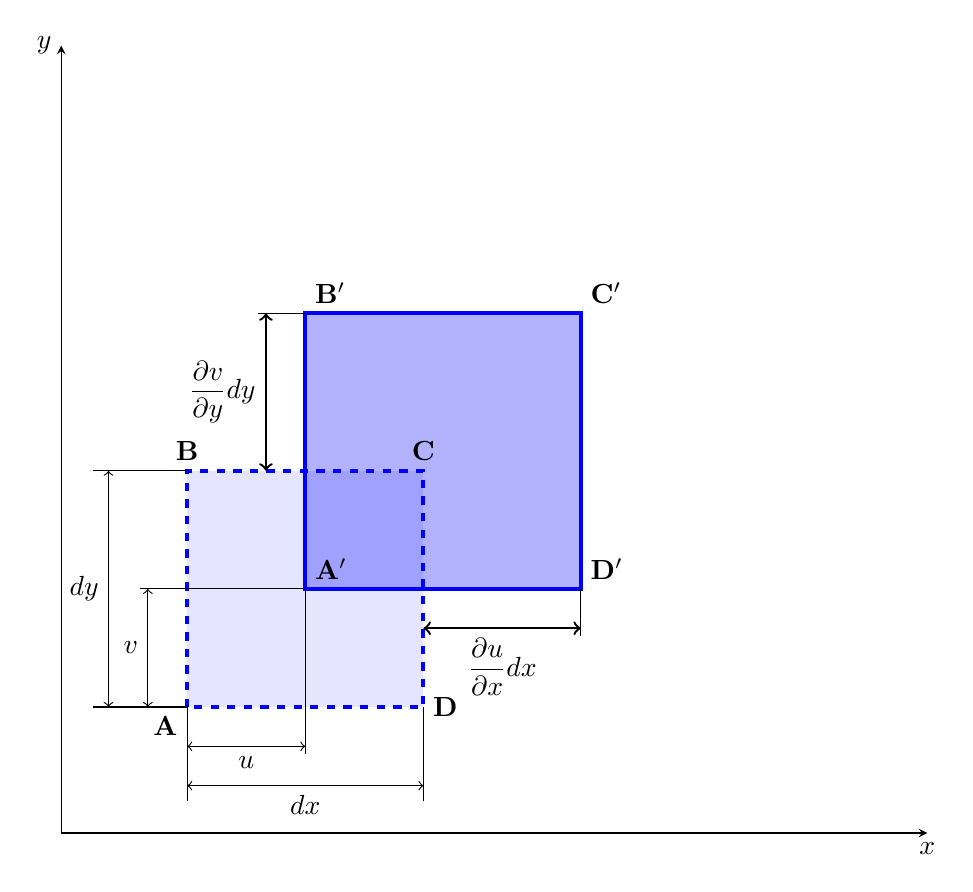
\begin{tikzpicture}
                \draw[-stealth] (0,0) -- (11,0) node[below]{$x$};
                \draw[-stealth] (0,0) -- (0,10) node[left]{$y$};
                \begin{scope}[transform canvas={xshift = 0.6cm, yshift = 0.6cm}]
                    \node (A) at (1,1) {};
                    \node (B) at (1,4) {};
                    \node (C) at (4,4) {};
                    \node (D) at (4,1) {};
                    \draw[line width = 0.5mm, dashed, blue, fill = blue, fill opacity = 0.1] (A.center) -- (B.center) -- (C.center) -- (D.center) -- cycle;
                    
                    
                    \node (A') at (2.5,2.5) {};
                    \node (B') at (2.5,6.0) {};
                    \node (C') at (6,6) {};
                    \node (D') at (6,2.5) {};
                    
        
                    \draw[line width = 0.5mm, blue, fill = blue, fill opacity = 0.3]  (A'.center) -- (B'.center) -- (C'.center) -- (D'.center) -- cycle;
        
                    \draw node[below left] at (A.center) {$\mathbf{A}$};
                    \draw node[above] at (B.center) {$\mathbf{B}$};
                    \draw node[above] at (C.center) {$\mathbf{C}$};
                    \draw node[right] at (D.center) {$\mathbf{D}$};
                    \draw node[above right] at (A'.center) {$\mathbf{A'}$};
                    \draw node[above right] at (B'.center) {$\mathbf{B'}$};
                    \draw node[above right] at (C'.center) {$\mathbf{C'}$};
                    \draw node[above right] at (D'.center) {$\mathbf{D'}$};
        
        
        
        
                    \draw[<->, transform canvas={xshift = -0.5cm}] (A.center)  -- (A'.center -| A.center) node[midway, left]{$v$};
                    \draw[<->, transform canvas={yshift = -0.5cm}] (A.center)  -- (A'.center |- A.center)  node[midway, below]{$u$};
                    
                    \draw[<->, transform canvas={yshift = -1cm}] (A.center)  -- (D.center |- A.center)  node[midway, below]{$dx$};
        
                    \draw[<->, transform canvas={xshift = -1cm}] (A.center)  -- (B.center -| A.center)  node[midway, left]{$dy$};
                    
        
                    \draw (A'.center -| A.center) ++ (-0.6,0) -- (A'.center) -- (A'.center |- A.center) --++ (0,-0.6);
                    \draw ({(-0.2,0)} |- A.center) -- (A.center) -- ({(0,-0.2)} -| A.center);
                    \draw ({(-0.2,0)} |- B.center) -- (B.center);
                    \draw ({(0,-0.2)} -| D.center) -- (D.center);
        
                    \draw[<->,  transform canvas={yshift = -0.5cm}, line width = 0.3mm] (C.center |- A'.center) -- (D'.center) node[midway, below]{$\displaystyle \frac{\partial u}{\partial x} dx$};
                    \draw (D'.center) --++ (0,-0.6);
                    
                    \draw[<->,  transform canvas={xshift = -0.5cm}, line width = 0.3mm] (C.center -| A'.center) -- (B'.center) node[midway, left]{$\displaystyle \frac{\partial v}{\partial y} dy$};
                    \draw (B'.center) --++ (-0.6,0);
        
        
                \end{scope}
            \end{tikzpicture}
        }
        \caption{deformação linear}
        \label{fig:deformacao_elemento_1}
    \end{subfigure}
    \begin{subfigure}[b]{0.45\textwidth}
        \resizebox{\textwidth}{!}{
            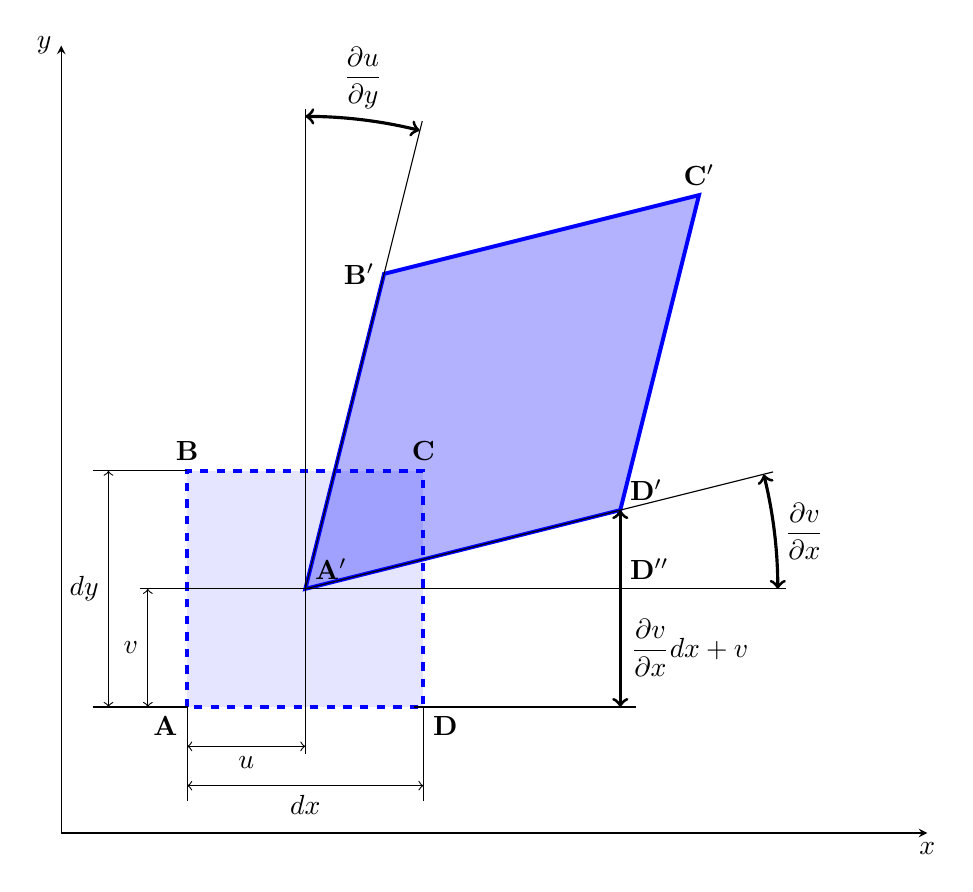
\begin{tikzpicture}
                \draw[-stealth] (0,0) -- (11,0) node[below]{$x$};
                \draw[-stealth] (0,0) -- (0,10) node[left]{$y$};
                \begin{scope}[transform canvas={xshift = 0.6cm, yshift = 0.6cm}]
                    \node (A) at (1,1) {};
                    \node (B) at (1,4) {};
                    \node (C) at (4,4) {};
                    \node (D) at (4,1) {};
                    \draw[line width = 0.5mm, dashed, blue, fill = blue, fill opacity = 0.1] (A.center) -- (B.center) -- (C.center) -- (D.center) -- cycle;
                    
                    
                    \node (A') at (2.5,2.5) {};
                    \node (B') at (3.5,6.5) {};
                    \node (C') at (7.5,7.5) {};
                    \node (D') at (6.5,3.5) {};
                    
        
                    \draw[line width = 0.5mm, blue, fill = blue, fill opacity = 0.3]  (A'.center) -- (B'.center) -- (C'.center) -- (D'.center) -- cycle;
        
                    \draw node[below left] at (A.center) {$\mathbf{A}$};
                    \draw node[above] at (B.center) {$\mathbf{B}$};
                    \draw node[above] at (C.center) {$\mathbf{C}$};
                    \draw node[below right] at (D.center) {$\mathbf{D}$};
                    \draw node[above right] at (A'.center) {$\mathbf{A'}$};
                    \draw node[left] at (B'.center) {$\mathbf{B'}$};
                    \draw node[above] at (C'.center) {$\mathbf{C'}$};
                    \draw node[above right] at (D'.center) {$\mathbf{D'}$};
        
        
                    \draw[<->, transform canvas={xshift = -0.5cm}] (A.center)  -- (A'.center -| A.center) node[midway, left]{$v$};
                    \draw[<->, transform canvas={yshift = -0.5cm}] (A.center)  -- (A'.center |- A.center)  node[midway, below]{$u$};
                    
                    \draw[<->, transform canvas={yshift = -1cm}] (A.center)  -- (D.center |- A.center)  node[midway, below]{$dx$};
        
                    \draw[<->, transform canvas={xshift = -1cm}] (A.center)  -- (B.center -| A.center)  node[midway, left]{$dy$};
                    
        
                    \draw (A'.center -| A.center) ++ (-0.6,0) -- (A'.center) -- (A'.center |- A.center) --++ (0,-0.6);
                    \draw ({(-0.2,0)} |- A.center) -- (A.center) -- ({(0,-0.2)} -| A.center);
                    \draw ({(-0.2,0)} |- B.center) -- (B.center);
                    \draw ({(0,-0.2)} -| D.center) -- (D.center);
        
        
                    
                    \draw (A'.center) -- (A'.center |- C') --++ (0,1.1);
                    \draw (A'.center) -- (A'.center -| C') --++ (1.1,0);
        
                    \draw[shorten >= -2cm] (A'.center) -- (B'.center);
                    \draw[shorten >= -2cm] (A'.center) -- (D'.center);
        
                    \draw[<->, line width = 0.4mm]  (D'.center) -- (D' |- A.center) node[midway, below right]{$\displaystyle \frac{\partial v}{\partial x} dx + v$};
                    \draw (D.west) -- (D -| D') --++ (0.2,0);
        
                    
                    \draw[<->, line width = 0.4mm] (A'.center) ++ (6,0)  arc (0:14:6) node[midway, right]{$\displaystyle \frac{\partial v}{\partial x}$};
        
                    \draw[<->, line width = 0.4mm] (A'.center) ++ (0,6)  arc (90:76:6) node[midway, above]{$\displaystyle \frac{\partial u}{\partial y}$};
        
        
                    \draw (D' |- A') node[above right]{$\mathbf{D''}$};
                \end{scope}
            \end{tikzpicture}
        }
        \caption{deformação angular}
        \label{fig:deformacao_elemento_2}
    \end{subfigure}
    \label{fig:deformacao_elemento}
\end{figure}